\chapter{Timing}
\label{chap: timing}

\section{Framing the Objective}


With an understanding of the collection and storage of baseband data, we can move on to the question of timekeeping.
The primary issue we must overcome is the misalignment of the human-time clocks in each antenna. 
As mentioned in Chapter~\ref{chap:antenna}, each antenna has a drift-prone human-time clock.
Every time we fetch baseband data at a certain point in unix time, we encounter some unknown offset between 
when we think it was measured and when the data was actually measured.
This is problematic when computing visibilities, since extracting any useful interferometric information 
requires the two timestreams to be perfectly aligned.
However, each antenna also has an internal nano-second iterator, meaning each spectrum (discrete collection of such nano-second iterations)
is almost perfectly (for the purposes of this section) spaced. 
Thus, if we can find the exact offset in spectra between each antenna at a certain point, we know the exact offset 
for the entire day. 
Figure~\ref{fig:offset_diagram} illustrates this visually.
\begin{figure}[H]
    \centering
    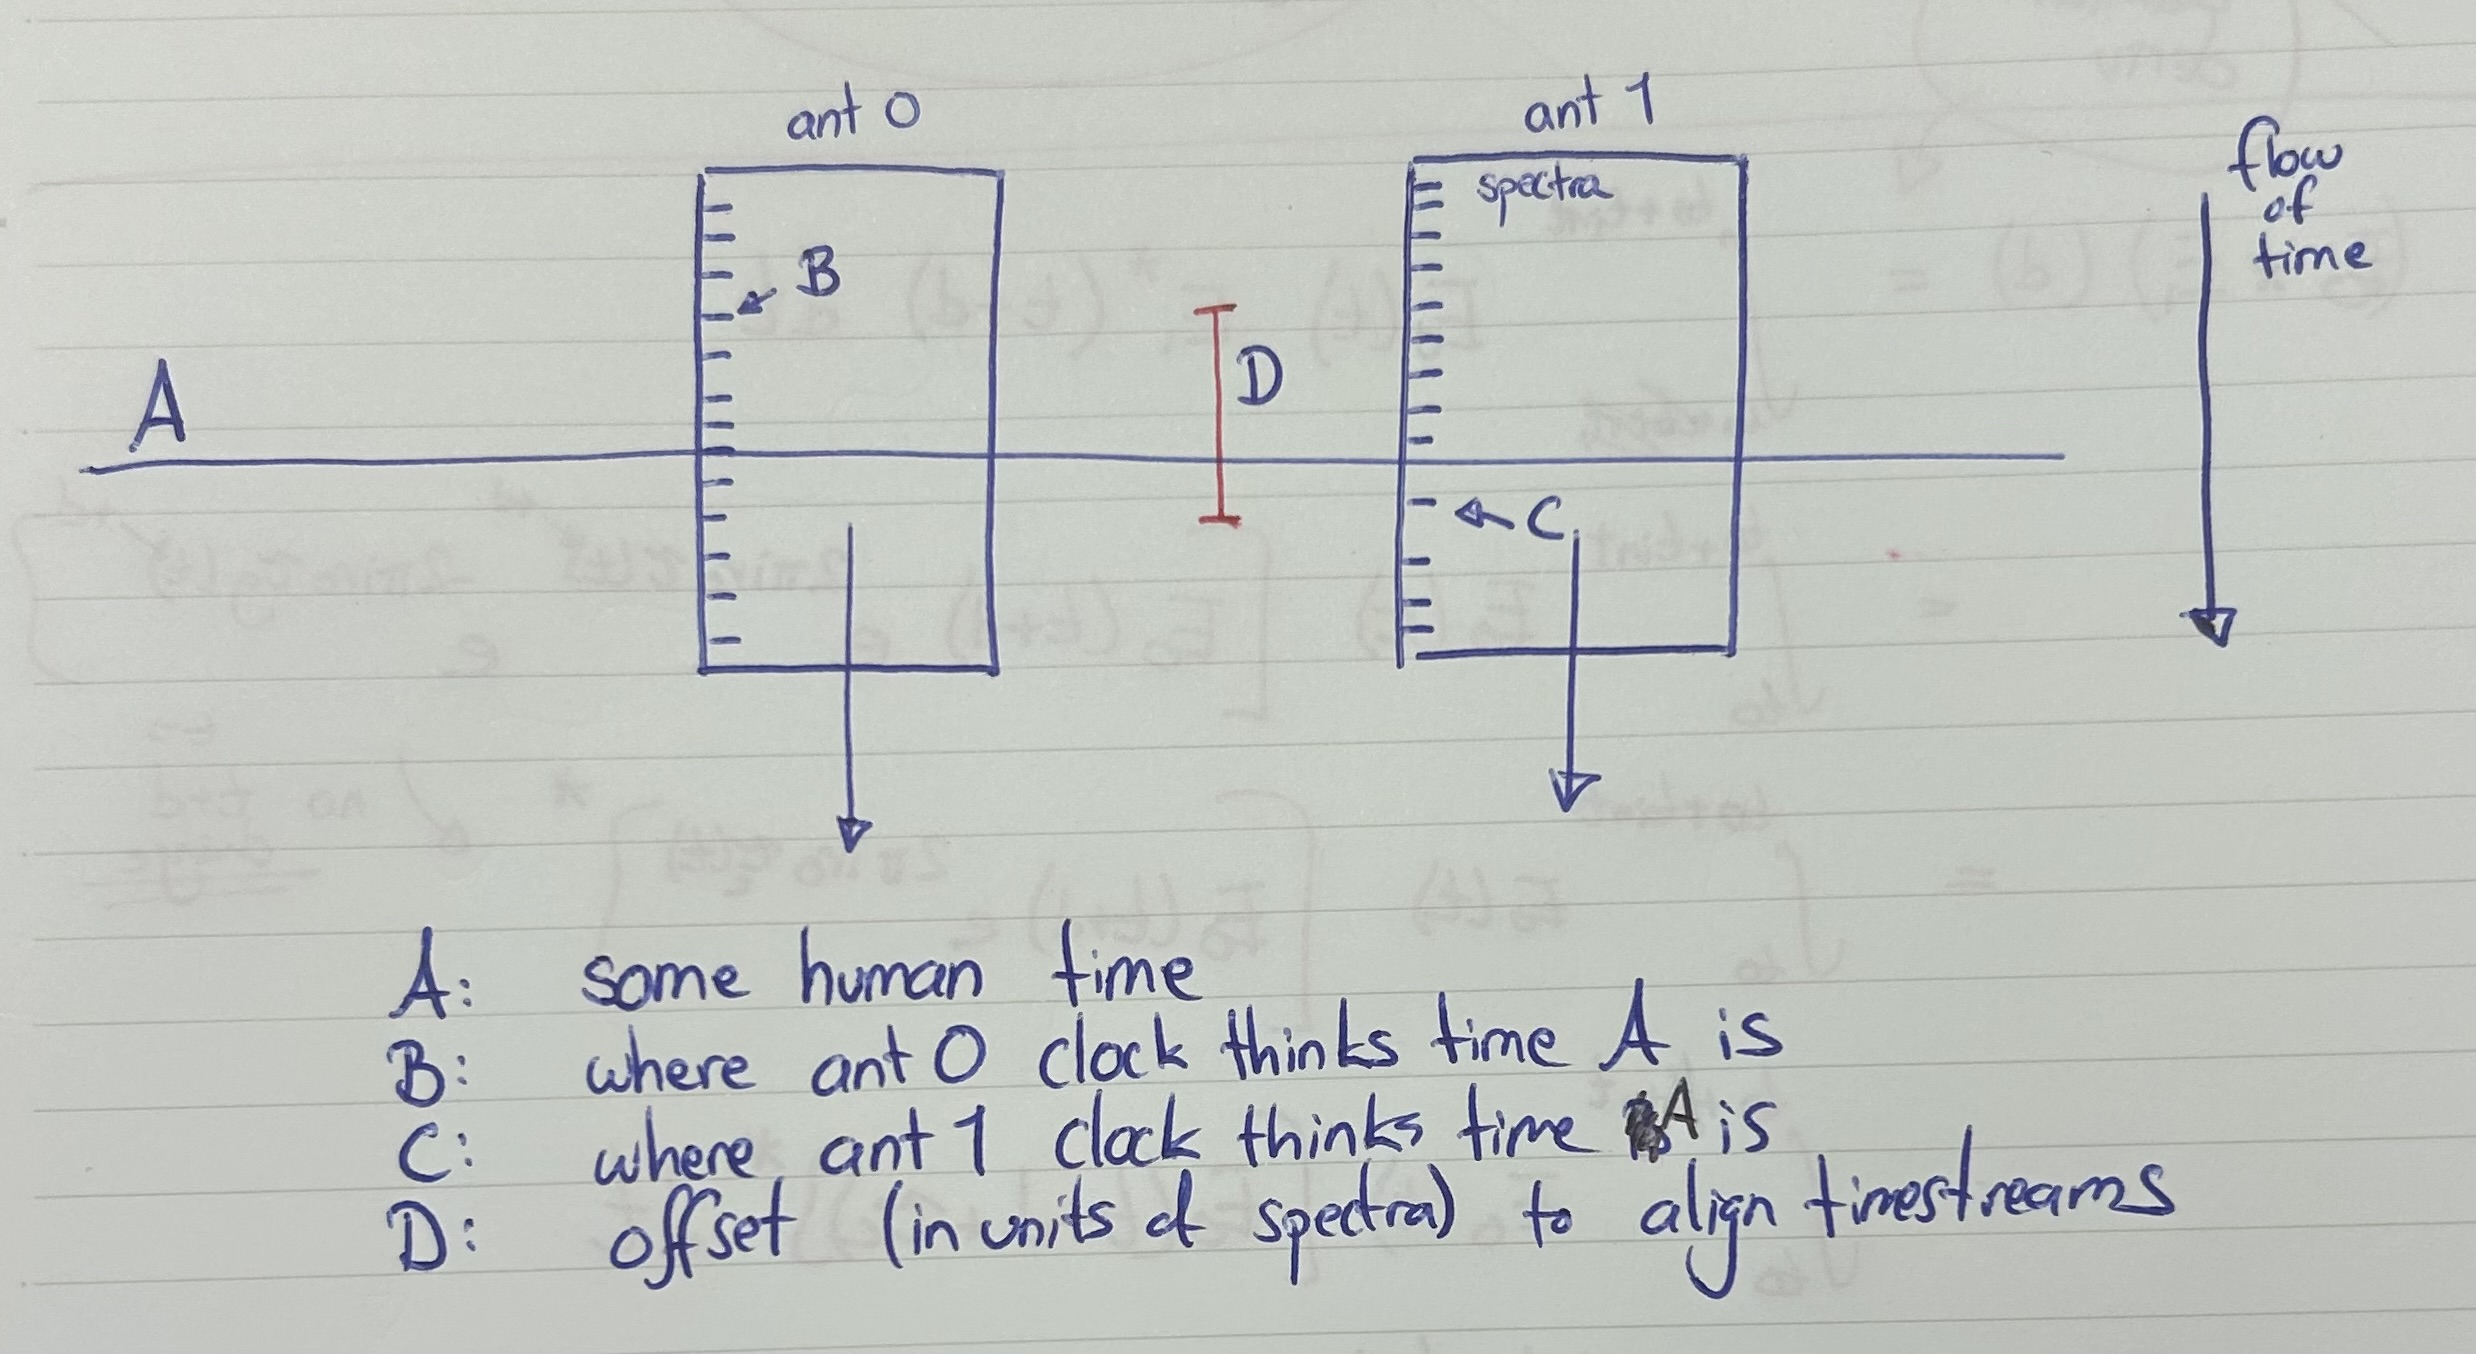
\includegraphics[width=0.7\linewidth]{Figures/offset_diagram.jpg}
    \caption{(Temporary!) Illustration of time offsets in Baseband data timestreams.}
    \label{fig:offset_diagram}
\end{figure}
Note that in this case, the exact observer time loses its significance, since all we really care about is the 
alignment between timestreams. 
We call this game of finding the spectrum index offset between antenna timestreams "spectrum number alignment".


As a side note, since spectra have some finite duration (about 16 $\mu s$ in our case), we cannot align the datastreams
to an infinite level of precision, rather simply to the closest spectrum number integer.  
Despite lacking perfect accuracy, it gives an excellent approximation of the clock offset, leading us into 
more precise corrections later in the analysis (see Chapter~\ref{chap:fine_timing}).


\section{Satellite Passes}

Spectrum number alignment relies on measuring some signal that is visible from both antenna. 
We require a source which: is bright to ensure high SNR, has a known position (for beamforming), 
and has some form of regularity for observation verification.
The best candidates are low orbit satellites, since their signals are strong, their positions are well documented and highly accurate, 
and each satellite passes overhead approximately every 90 minutes. 


Figure~\ref{fig:sat_pulse}   Let us visualize what a satellite pass looks like for two antenna.

\begin{figure}[H]
    \centering
    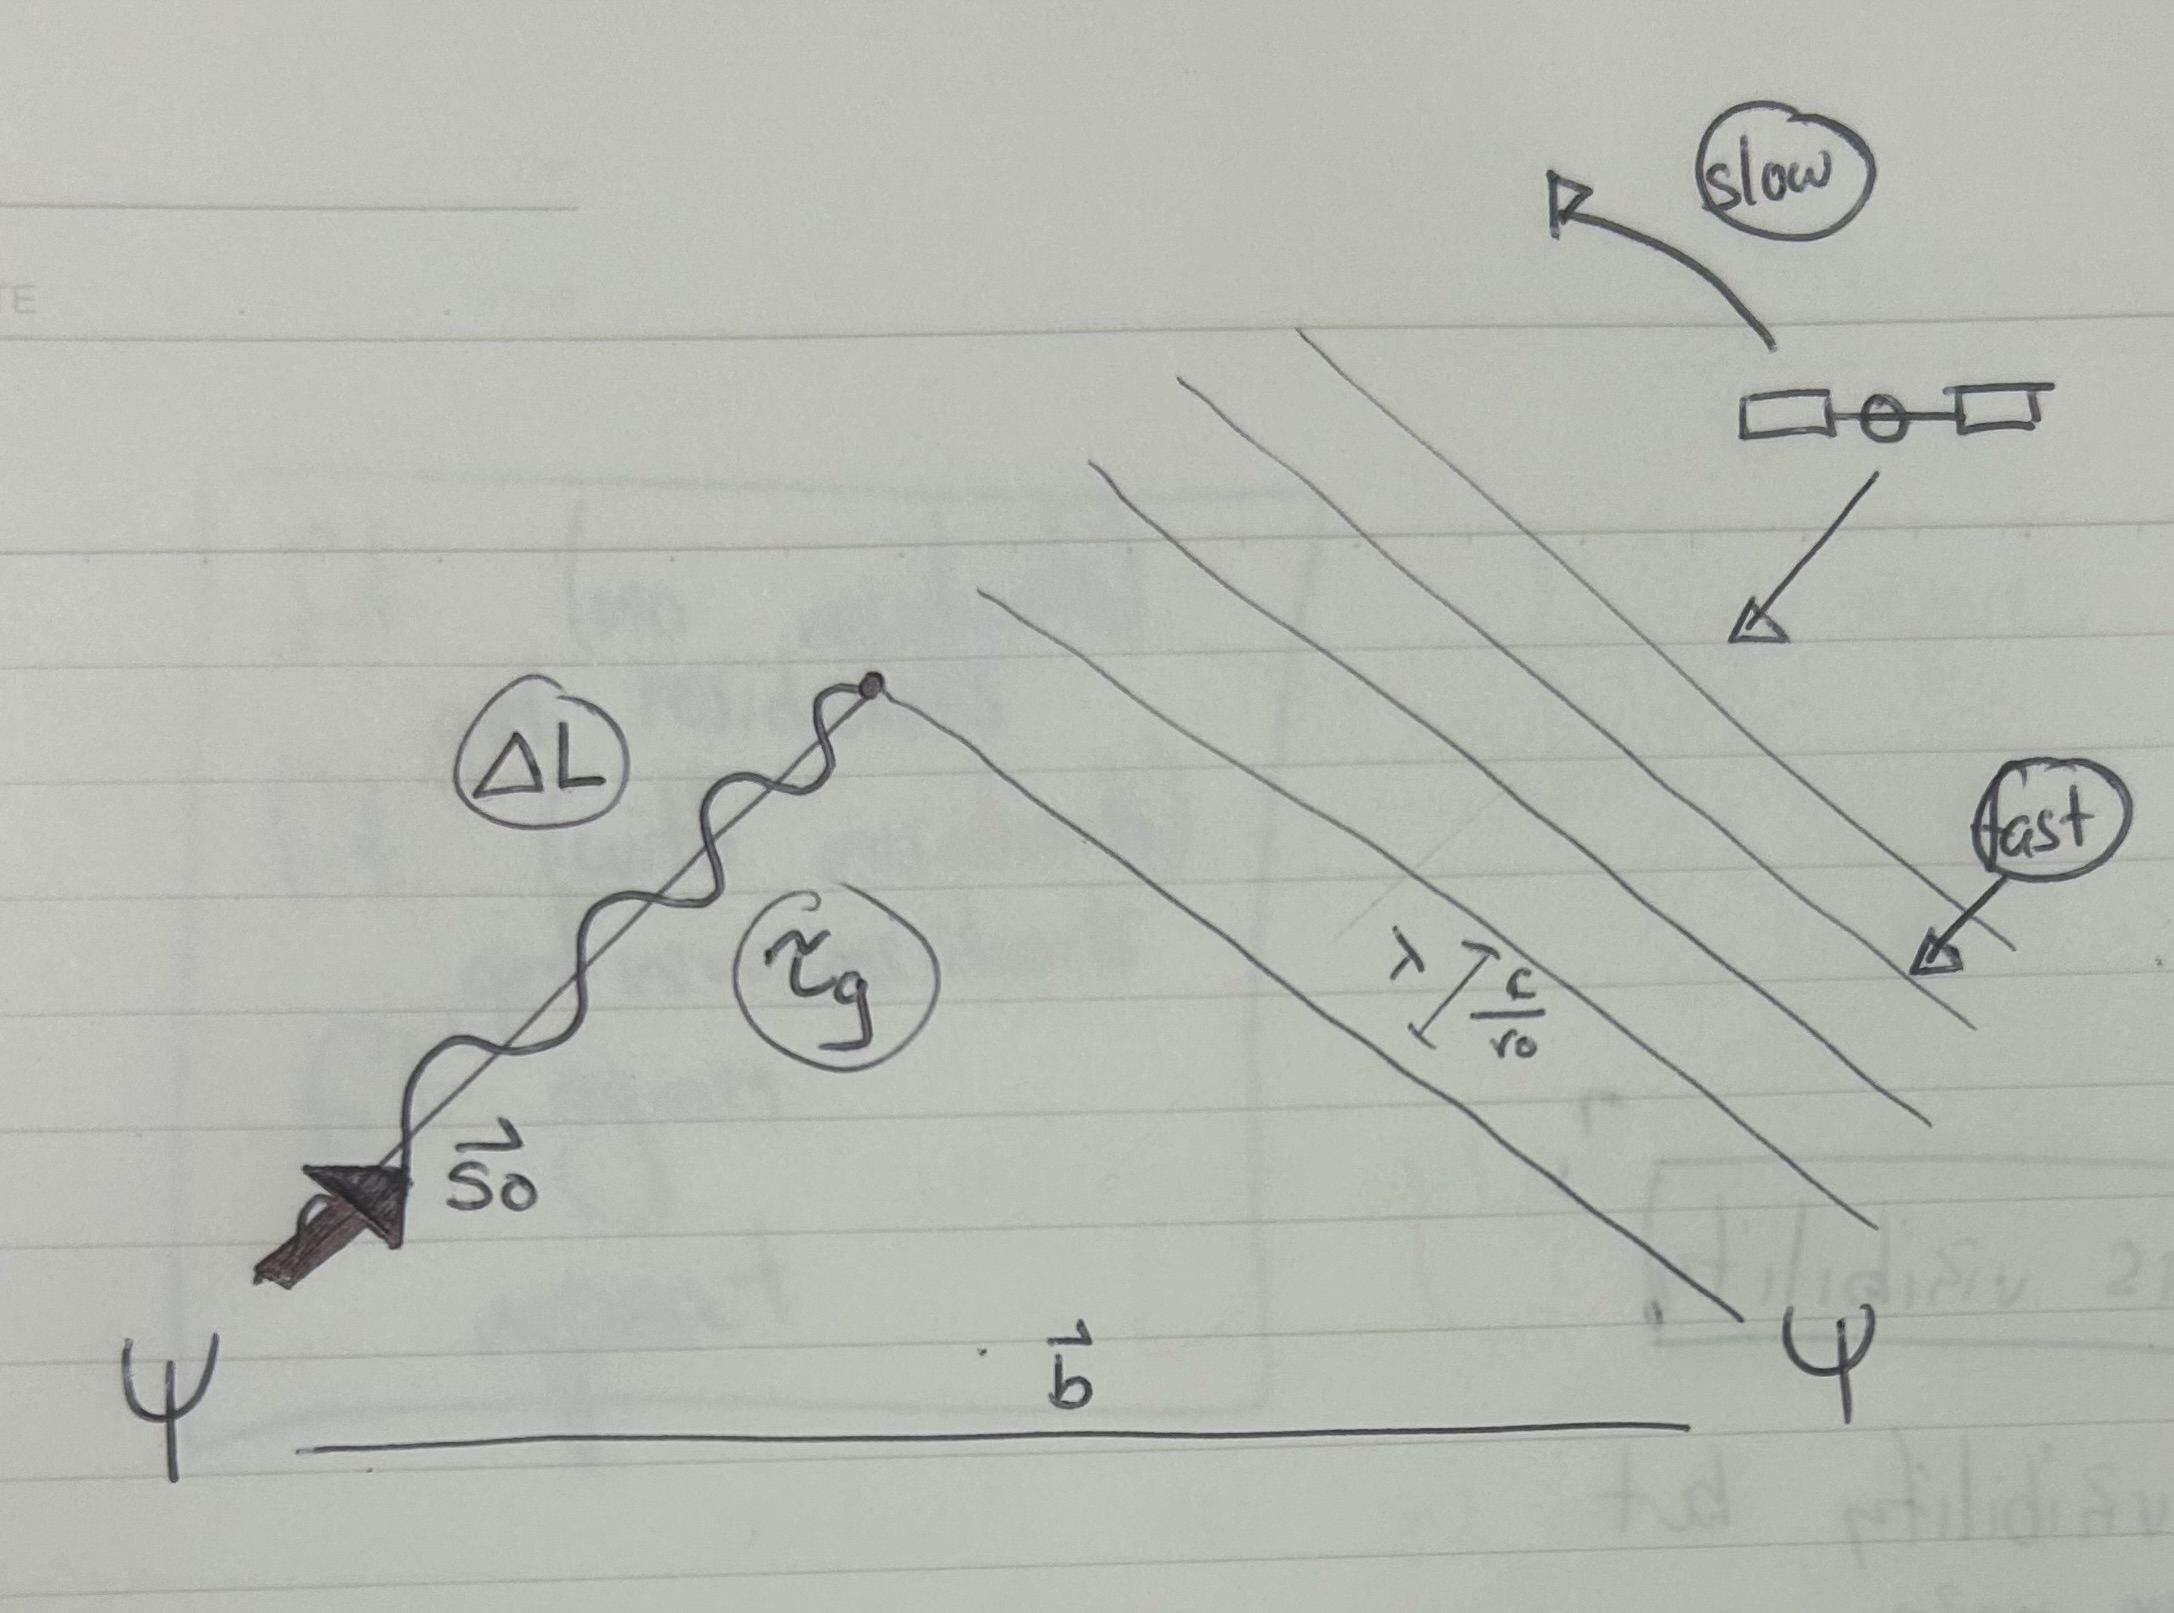
\includegraphics[width=0.7\linewidth]{Figures/sat_det_plot.jpg}
    \caption{(Temporary!) Illustration of a satellite pass}
    \label{fig:sat_pulse}
\end{figure}

Consider a very strong narrowband satellite signal at frequency channel $\nu_0$, in direction $\vec{s_0}$. 
Let us apply the flat sky approximation.
Let us also assume the satellite signal is far brighter than anything else the antenna sees,
such that the sky brightness function $I(\nu, \vec{s})$ is a delta function in the satellite's direction $\vec{s_0}$ 
and at its frequency $\nu_0$. 
We make no assumption on the brightness function in other channels.
Moreover, we also assume the antenna response is uniform.


Let's assume the electric field measured by Antenna 0 is a function of time, $E_0 (t) = a(t) e ^{2 \pi i \nu_0 t}$. 
As we can see in Figure~\ref{fig:sat_pulse}, there is a geometric delay ($\tau_g(t)$)
between the signal arriving at Antenna 0 and Antenna 1, caused by the angle of the satellite in the sky.
Note that $\tau_g(t)$ is a function of time as the satellite's position changes over the duration of its pulse. 
We let the clock offset between the antenna timestreams be $\tau_c(t)$, such that for the satellite signal, 
the total offset between the antenna data streams is $\tau(t) = \tau_c(t) + \tau_g(t)$.
Thus, the signal measured in the Antenna 1 timestream is $E_1 (t) = E_0 e^{2 \pi i \nu_0 \tau(t)}$. 


Our objective here is to find $\tau_c(t)$ given our knowledge of $\tau_g$ (which is easily derived from the satellite's position).
The general idea is removing $\tau_g$ by applying a phase to $E_1$, and then performing a coarse cross-correlation with 
several different spectrum number offsets. 
We are essentially beamforming our antenna towards the expected direction of the satellite, and searching for a signal response. 
The maximal absolute value of the coarse cross-correlation will be attained at the correct offset, as seen below:

\begin{eqnarray}
    (E_0*E_1)(\tau) &=& \int^{t_0 + t_{\text{int}}}_{t_0} E_0(t) E_1^*(t+\tau) dt, \\\nonumber
    &=& \int^{t_0 + t_{\text{int}}}_{t_0} E_0(t) {\left[ E_0(t+\tau) e^{-2\pi i \nu_0 \tau_g(t) + \tau_c(t)} e^{-2\pi i \nu_0 \tau_g(t) } \right]}^* , \\\nonumber
    &=& \int^{t_0 + t_{\text{int}}}_{t_0} E_0(t) {\left[ E_0(t + \tau + \tau_c) \right]}^ *, \\\nonumber
    &=& \int^{t_0 + t_{\text{int}}}_{t_0} E_0(t)  E_0^*(t + \tau + \tau_c)
\end{eqnarray}
Clearly, if $\tau = \tau_c$, we expect the maximal value of the absolute value of the integral, as $E_0$ is correlated with itself. 
It is important to note that we assume both $\tau_c(t)$ and $\tau_g(t)$ remain constant over the course of the cross-correlation.
In general, this holds as the accumulation length $t_{\text{acc}}$ is much smaller than the period of the phasor $e^{2\pi i \nu_0 \tau_g(t)}$.

This approach is a significant simplification of the method far better explained in a document by Mohan Agrawal, found here XX. 

 
As an aside, it is easy to confuse the application of a geometric delay (order 100ns) as being insignificant to a single spectrum
offset (order 16 $\mu s$).
So, why would the removal of 100ns affect a measurement made by shifting in units of 16 $\mu s$?
The geometric delay is better thought of as a phase which compensates for this path difference.
We can easily find the signal arrival's time difference between the antenna, which can be turned into the angle difference
$e^{2 i \pi f \tau_g}$ between the two antenna.
This angle compensation is akin to tilting the (so to say) direction of focus of the antenna.

It is also important to consider that this derivation only holds for the narrowband limit, since a real signal
contains many frequencies. 
Offsets are not quite as simply added for such layered signals.



\section{Practical Implementation}

\subsection{Nomenclature}

Before any correlation can be done, we require accurate and reliable satellite position information. 
The first step of detection is knowing what satellites the antenna can see.
If we know that a satellite is in the field of view of the antenna, we say it is \textbf{risen}. 
The duration over which this satellite is risen is referred to as a \textbf{pass}. 
However, not all risen satellites are visible in the satellite data. 
If we can find the satellite in the correlation of the antenna data, we say it is \textbf{detected}, 
and the duration of time it is risen is a \textbf{pulse}, since we observe a peak in the data for these times. 
Our analysis therefore starts with a long list of risen satellites, with their pass times and satellite ID. 
We aim to detect these. 

Next, TLE files allow us to calculate the geometric delay between the antenna using this TLE file data.
Moreover, if there are multiple satellites present in the pass, applying the different expected geometric delays helps 
differentiate between them.

Thus, we can find a period of data where we know a satellite is risen, and know exactly what the geometric delay is at that time.


\subsection{Discrete Computation}

In practice, spectrum number alignment is done by discrete coarse cross correlation.
We take a chunk of $10^6$ spectra, and consider the central XXXXX spectra.
Since we are shifting the data, we need a buffer such that we don't run out of data for the offset timestream.
We shift the two timestreams by up to 100 000 spectra in either direction, each time correlating these XXXX spectra.
Thus, we end up with 200 001 different correlations (where the extra correlation comes from the zero-offset),
each corresponding to a different spectrum number offset.
Below is the discrete version of one single such correlation, for spectrum number offset k.

\begin{eqnarray}
    (E_0*E_1)(k) &=& \sum_{n=-N}^N E_0[k]E_1^*[n+k]
\end{eqnarray}

Here $N$ is the maximum spectrum offset we will go to, so $N=100000$. 
Figure~\ref{fig:sat_cxcorr_example} shows an example of such a coarse cross-correlation.


\begin{figure}[H]
    \centering
    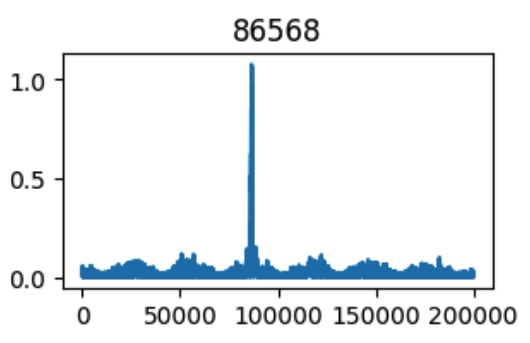
\includegraphics[width=0.5\linewidth]{Figures/american_1.jpeg}
    \caption{A typical cross-correlation for a satellite pass. The x-axis indices are actually -100000 to 100000, 
    matplotlib has just indexed them with natural numbers. The title gives the correlation offset index, 86568, which corresponds to 
    a spectrum number offset of -13432} 
    \label{fig:sat_cxcorr_example}
\end{figure}

There is a clear peak, but as we will later see, this peak may be ambiguous.
Moreover, it is important to realize the spectrum number offset between the antenna, -13432, gives the difference between expected
and measured antenna spectra. 
However, the actual global indices of the antenna are different, and must be adjusted by this value.
For example, let's say the baseband data tells us that at 4pm, Antenna 0 is at spectrum 100000, Antenna 1 is at spectrum 200000, 
and we found an offset of -13432. 
Our convention is that offsets are Ant0 - Ant1, so we know the adjusted global spectrum number offset is 113432.


\section{Analyzing Pulses}

Unfortunately, not all pulses are born equal. 
It turns out that US NORAD satellites have ambiguous peaks, making the spectrum number offset alignment a relatively noisy 
value when considering multiple pulses.
Figure~\ref{fig:american_sats} shows a typical American satellite pulse.


\begin{figure}[H]
    \centering
    \begin{subcaptionbox}{Image 1\label{fig:image1}}[0.3\textwidth]
        {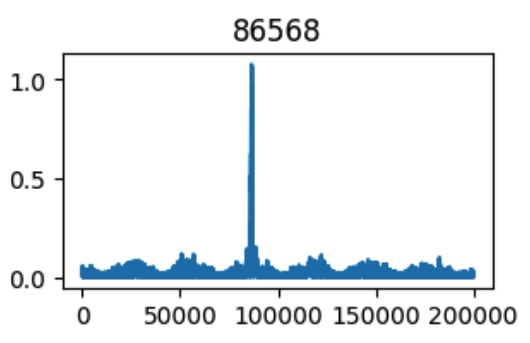
\includegraphics[width=\linewidth]{Figures/american_1.jpeg}}
    \end{subcaptionbox}
    \hfill
    \begin{subcaptionbox}{Image 2\label{fig:image2}}[0.3\textwidth]
        {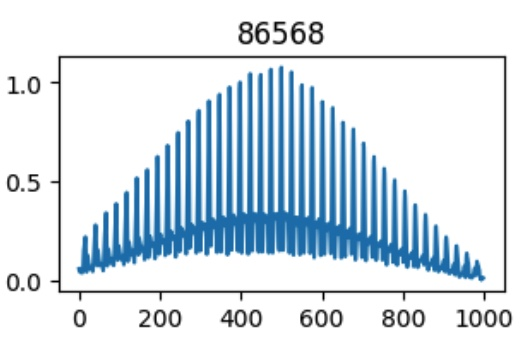
\includegraphics[width=\linewidth]{Figures/american_2.jpeg}}
    \end{subcaptionbox}
    \hfill
    \begin{subcaptionbox}{Image 3\label{fig:image3}}[0.3\textwidth]
        {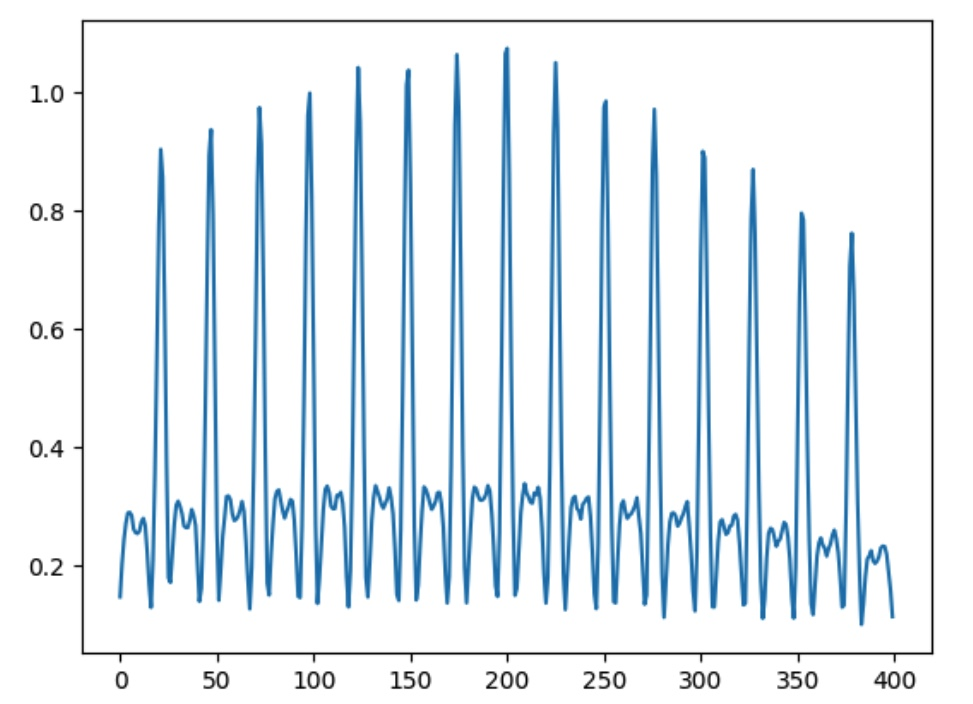
\includegraphics[width=\linewidth]{Figures/american_3.jpeg}}
    \end{subcaptionbox}
    \caption{A usual American satellite pulse. Left is most zoomed out, right is most zoomed in. Can see the periodic peaks.}
    \label{fig:american_sats}
\end{figure}

At high resolution, the peak consists of several smaller, sharp peaks. This means the offset can often get confused.

Fortunately, Russian satellites have a strong and distinct pulse in the coarse cross correlation, as seen in Figure~\ref{fig:russian_sats}.


%\begin{figure}[H]
%    \centering
%   \begin{subcaptionbox}{Image 1\label{fig:image1}}[0.3\textwidth]
%        {\includegraphics[width=\linewidth]{image1.jpg}}
%    \end{subcaptionbox}
%    \hfill
%    \begin{subcaptionbox}{Image 2\label{fig:image2}}[0.3\textwidth]
%        {\includegraphics[width=\linewidth]{image2.jpg}}
%    \end{subcaptionbox}
%    \hfill
%    \begin{subcaptionbox}{Image 3\label{fig:image3}}[0.3\textwidth]
%        {\includegraphics[width=\linewidth]{image3.jpg}}
%    \end{subcaptionbox}
%    \caption{A usual Russian satellite pulse. Left is most zoomed out, right is most zoomed in. Can see the sharp peak.}
%    \label{fig:three_images}
%\end{figure}
 
Clearly, such Russian peaks are far better for spectrum number alignment.
We can differentiate between them using what we call a \textbf{reliability ratio}.
This crude but effective method provides a measure of the sharpness of the peak.
It zooms into the closest 200 spectra from the main peak and finds the position of the five next-tallest peaks.
It then find the mean (normalized) difference between the main peak and the other next-tallest peaks.
If this value is high, then there are likely other similarly sized peaks bunched together, indicating an American-style pulse.
If this value if low, then there is only a single dominant peak, and we can trust the offset value it provides.
The reliability ratio is recorded alongside all other pulse information in the detection process.





